

\section{Background}\label{sec:background}

In this section, we present the background of Smart SSDs (Section~\ref{sec:SSDInternals}) and Lucene's search architectures (Section~\ref{sec:searchEngineArch}).
\subsection{Smart SSDs}\label{sec:SSDInternals}
The Smart SSD ecosystem consists of both hardware (Section~\ref{sec:SSDhw}) and software components (Section~\ref{sec:softArch}) to execute user-defined programs.
\subsubsection{Hardware Architecture}\label{sec:SSDhw}

\begin{figure}[htbp]
  \centering
  \begin{tabular}{ccc}
 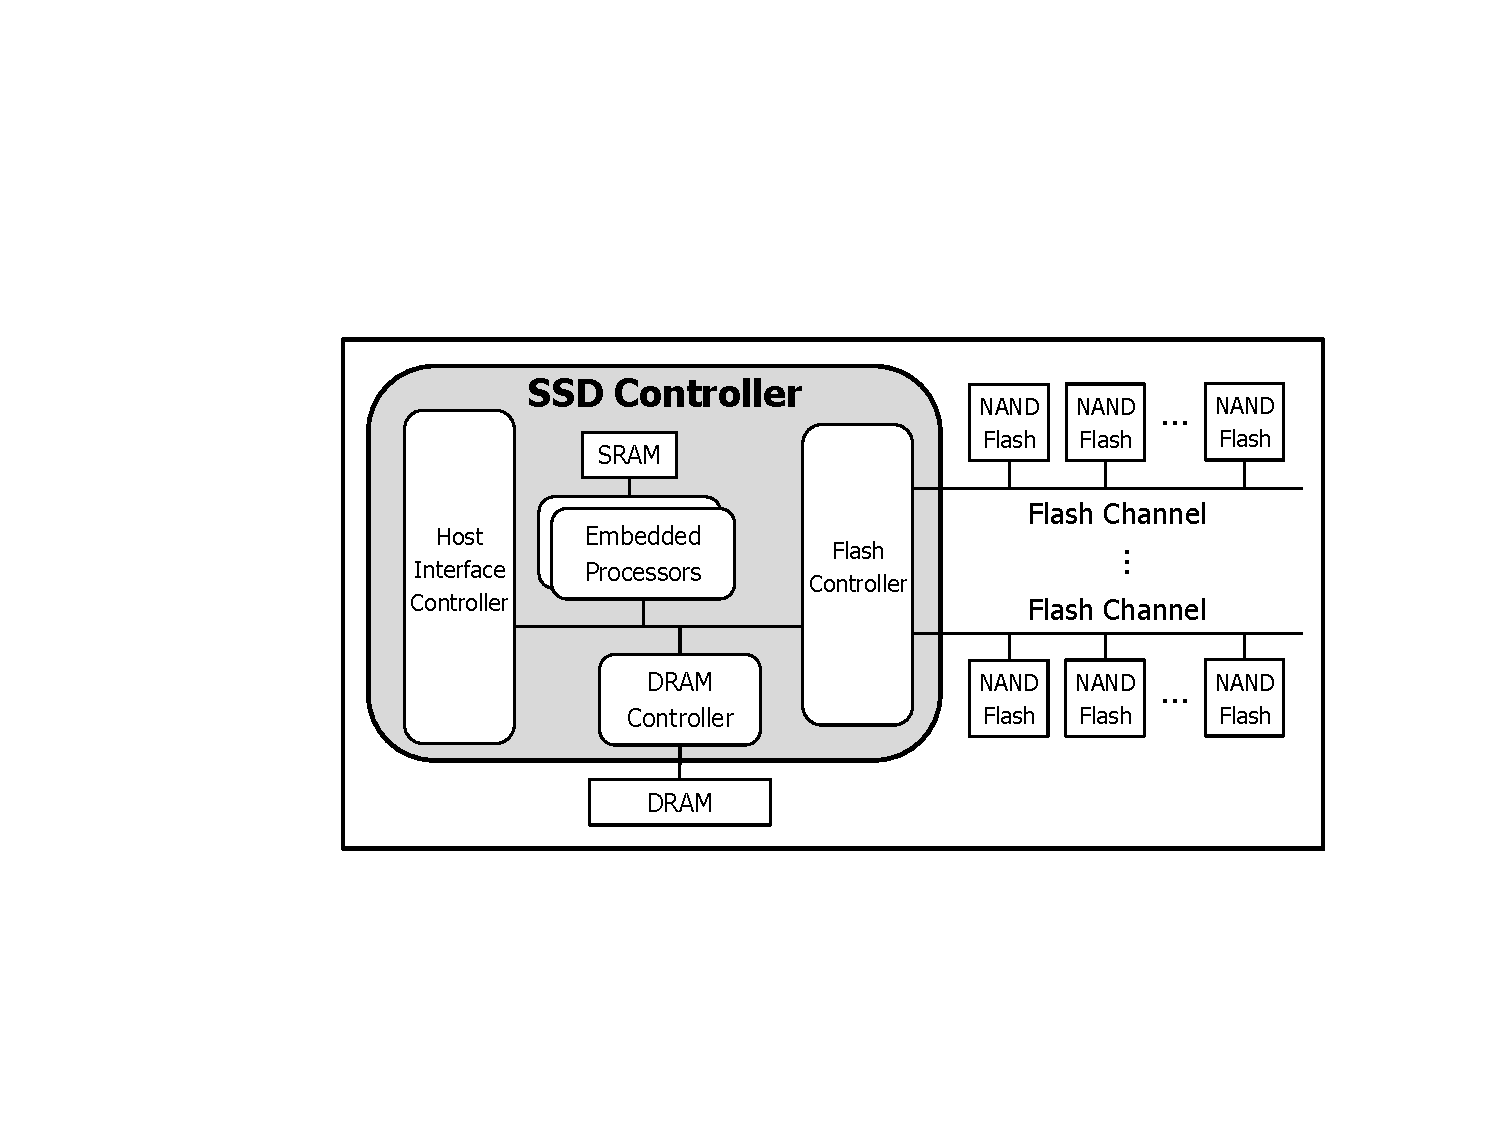
\includegraphics[width=0.95\columnwidth]{figures/SSDInternals.pdf}
\end{tabular}
  \caption{Smart SSD hardware architecture}
  \label{fig:SSDInternals}
 \end{figure}


Figure~\ref{fig:SSDInternals} represents the hardware architecture of the Smart SSD. The hardware architecture of Smart SSDs is similar to regular SSDs.
In general, an SSD is largely composed of NAND flash memory array, SSD controller, and (device) DRAM. The SSD controller is subdivided into four main subcomponents: host interface controller, embedded processors, DRAM controller, and flash controller.

The host interface controller processes commands from interfaces (typically SAS/SATA or PCIe) and distributes them to the embedded processors.
%Commands come from a user through the host interface and the most common interfaces, for instance, Serial ATA (SATA), Serial Attached SCSI (SAS), or PCI Express (PCIe), are implemented by the host interface controller.
The embedded processors receive the commands and pass them to the flash controller. More importantly, they run SSD firmware code for computation and execute Flash Translation Layer (FTL) for logical-to-physical address mapping~\cite{Chung2009SFT}. Typically, the processor is a low-powered 32-bit processor such as an ARM series processor. Each processor can have a tightly coupled memory (e.g., SRAM) to store performance-critical data or code. Each processor can access DRAM through the DRAM controller. The flash controller controls data transfer between flash memory and DRAM.

%For data transfer between flash memory and DRAM, the Flash Controller, also called Flash Memory Controller (FMC), is adopted. The FMC runs Error Correction Code (ECC) and supports Direct Memory Access (DMA) functionality.

%The NAND flash memory package (also called chip) is persistent storage media and each package consists of one or more dies. The die is the smallest unit that can independently execute commands or report status. Each die contains one or more planes (usually one or two). Identical or concurrent operations can take place on each plane, although with some restrictions. Each plane subdivides into a number of blocks which are the smallest erase unit, and finally each block is composed of many pages (typically 64 or 128 pages)which are the smallest read/write unit.
The NAND flash memory package is the persistent storage media and each package is subdivided further into smaller units that can independently execute commands or report status.
%An SSD is also equipped with a large size of DRAM for buffering data or storing metadata of the address mapping. All the flash channels share access to the DRAM. Thus, data transfer from the flash channels to the DRAM needs to be serialized.

\subsubsection{Software Architecture}\label{sec:softArch}

%Smart SSDs, unlike the traditional CPU-centric computing systems, enable ISC devices to play a major role in computation by offloading key functions of host systems into ISC devices. Since its hardware architecture is identical to the aforementioned modern SSDs shown in Figure~\ref{fig:SSDInternals}, this section describes our Smart SSD software architecture and key components as ISC devices.

In addition to the hardware support, we also need a software mechanism to define a set of protocols such that host machines and Smart SSDs can communicate with each other. Figure~\ref{fig:SmartSSD_arch} describes our Smart SSD software architecture which consists of two main components: \emph{Smart SSD firmware} inside the SSD and \emph{host Smart SSD program} in the host system.
The host Smart SSD program communicates with the Smart SSD firmware through application programming interfaces (APIs).




\begin{figure}[tbp]
%\vspace{-5mm}
	\centering
		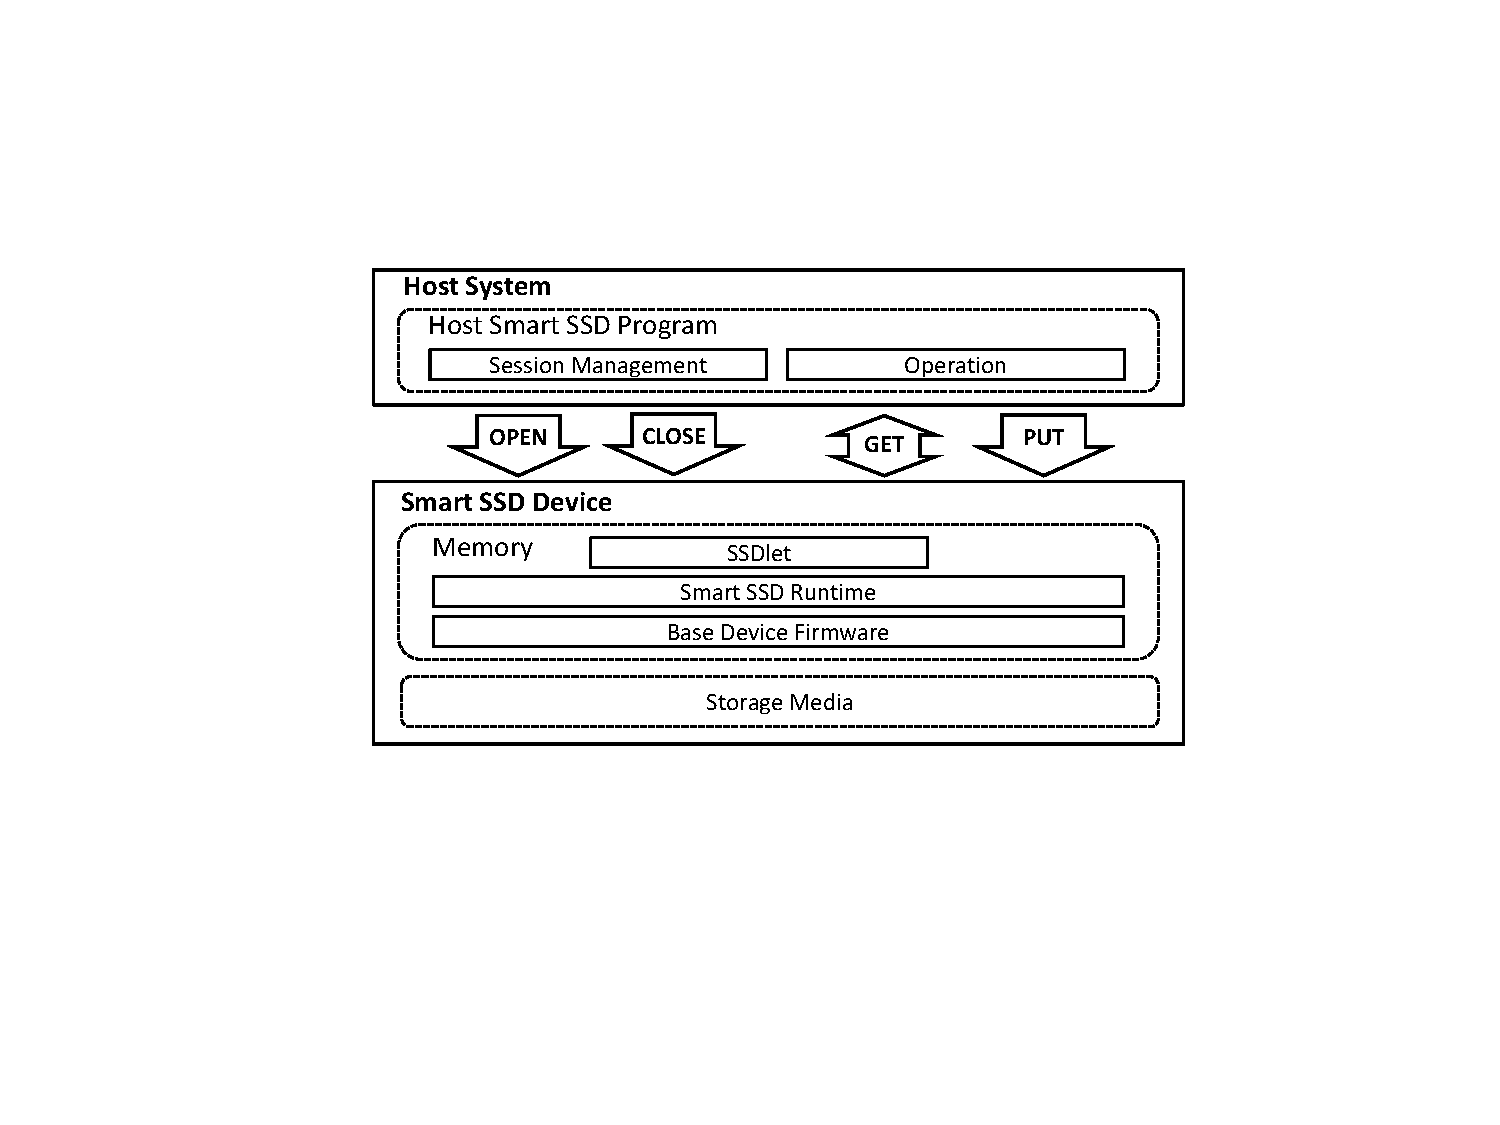
\includegraphics[width=0.95\columnwidth]{figures/SmartSSD_Architecture.pdf}
	\caption{Smart SSD software architecture}
	\label{fig:SmartSSD_arch}
\end{figure}

%As illustrated in Figure~\ref{fig:SmartSSD_arch}, our Smart SSD consists of several key software components and it communicates with a Smart SSD host program via Smart SSD application programming models (APIs).

The Smart SSD firmware is subdivided into three subcomponents: SSDlet, Smart SSD runtime, and base device firmware.
An SSDlet is a Smart SSD program in the SSD. It implements application logic and responds to a Smart SSD host program. The SSDlet is executed in an event-driven manner by the Smart SSD runtime system. A Smart SSD runtime system connects the device Smart SSD program with a base device firmware, and implements the library of Smart SSD APIs. In addition, a base device firmware also implements normal I/O operations (read and write) of a storage device.

%After an SSDlet is installed in the Smart SSD device, a host system runs the Smart SSD host program to interact with the SSDlet in the devices.
This host Smart SSD program consists largely of two components: a session management component and an operation component. The session component manages the lifetime of a session for Smart SSD applications so that the host Smart SSD program can launch an SSDlet by opening a session to the Smart SSD device. To support this session management, Smart SSD provides two APIs, namely, OPEN and CLOSE. Intuitively, OPEN starts a session and CLOSE terminates a session. Once OPEN starts a session, runtime resources such as memory and threads are assigned to run the SSDlet and a unique session ID is returned to the host Smart SSD program. Afterwards, this session ID must be associated to interact with the SSDlet. When CLOSE terminates the established session, it releases all the assigned resources and closes SSDlet associated with the session ID.

Once a session is established by OPEN, the operation component helps the host Smart SSD program interact with SSDlet in a Smart SSD device with GET and PUT APIs. This GET operation is used to check the status of SSDlet and receive output results from the SSDlet if the results are ready. This GET API implements the polling mechanism of the SAS/SATA interface because, unlike PCIe, such traditional block devices cannot initiate a request to a host such as interrupts. PUT is used to internally write data to the Smart SSD device without help from local file systems.


\subsection{Query Processing of Lucene}\label{sec:searchEngineArch}

\begin{figure}[htbp]
  \centering
  \begin{tabular}{ccc}
 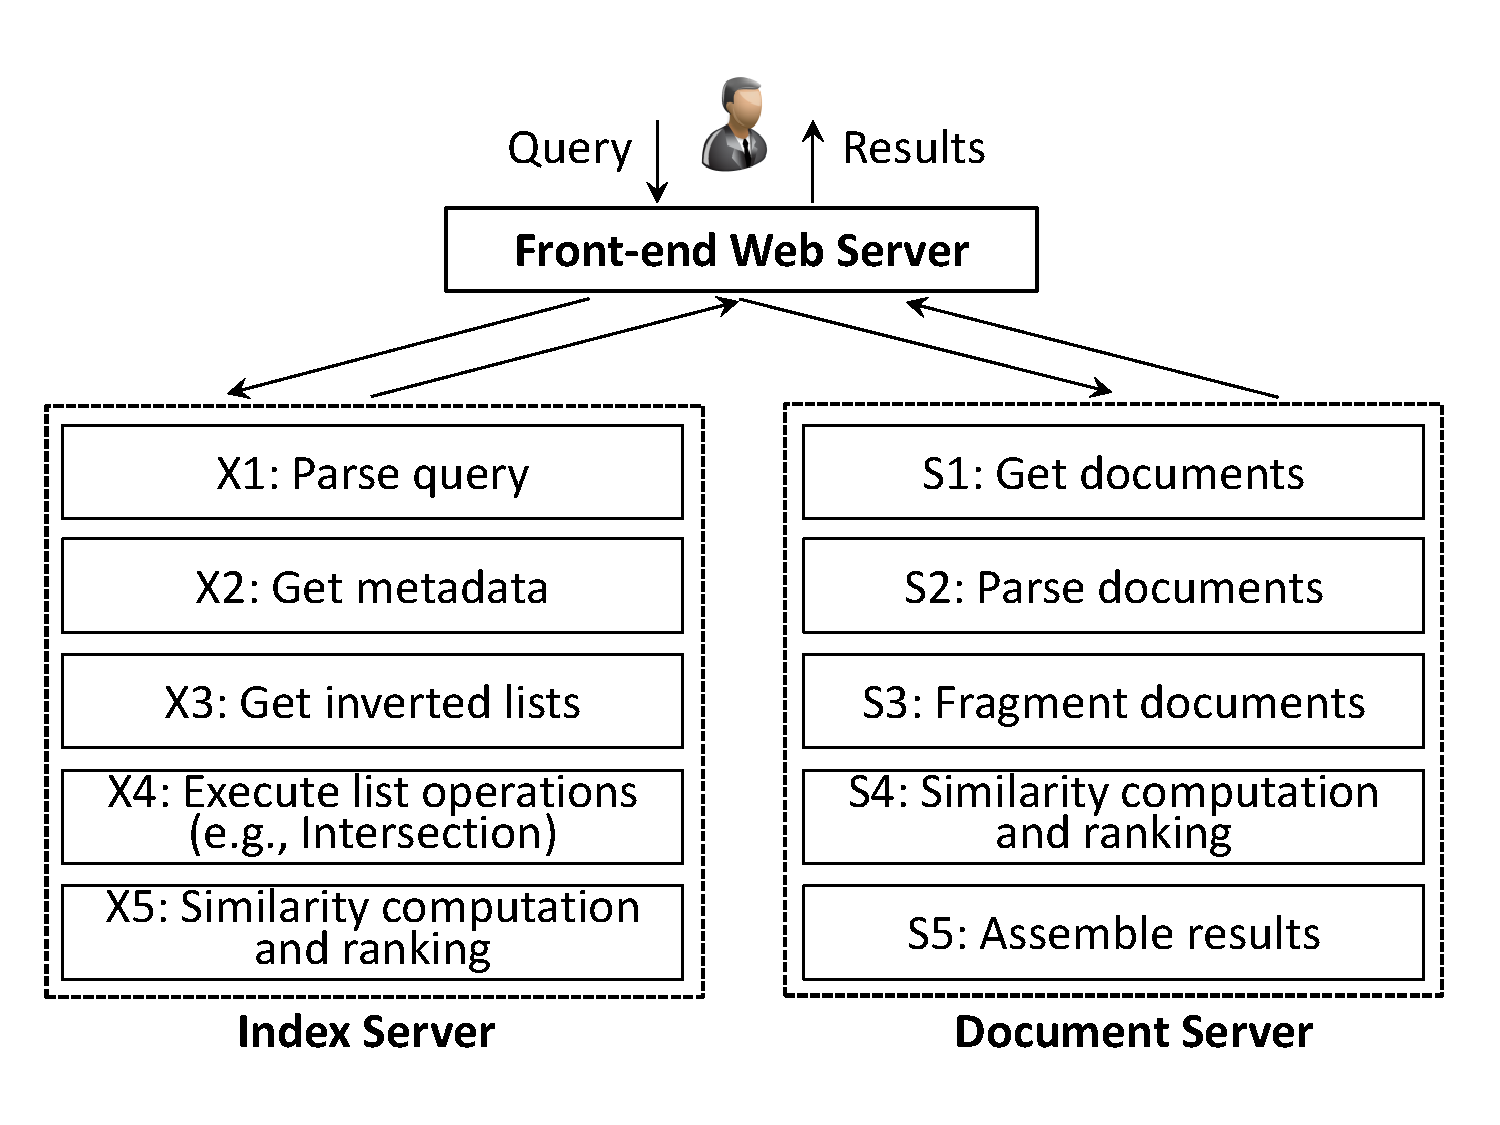
\includegraphics[width=0.4\columnwidth]{figures/searchEngineArch.pdf}
\end{tabular}
  \caption{Query processing of Lucene}
  \label{fig:searchEngineArch}
 \end{figure}

%Lucene is a well known open-source search engine and widely adopted in industry. E.g., LinkedIn~\cite{Hien2013} and and Twitter~\cite{Busch2012ERS} adopted Lucene in their search platforms.

%We provide some background of how a query is executed in Lucene.
Like other search engines, Lucene relies on the standard inverted index \cite{ZM06} to answer user queries efficiently. The inverted index is essentially a mapping data structure of key-value pairs, where the key is a query term and the value is a list of documents containing the term.

Upon receiving a user query $q$ (e.g., ``SSD database''), Lucene answers it through several steps (S1 to S5 in Figure~\ref{fig:searchEngineArch}).
\emph{Step S1}: Parse the query $q$ into query terms. In our example, there are two query terms: ``SSD'' and ``database''.
%Each node is a Lucene-defined query type. The root node is a conjunction query. Each leaf node is a term query.
%Each node is a Lucene-defined query type. The root node is a conjunction query, which returns the intersected results returned by the leaf nodes. Each leaf node is a term query, which returns a list of documents that contain that term, by referring to the inverted index.
\textit{Step S2}: get metadata for each query term. The metadata is used to load the inverted list of each query term in the next step. Thus, this metadata stores some basic information about the on-disk inverted list. In Lucene, it contains (1) the offset where the list is located on disk, (2) the list length (in bytes), and (3) the number of entries in the list.
\textit{Step S3}: for each term, get the inverted list from disk to memory.
\textit{Step S4}: execute list operations depending on query modes.
By default, Lucene enables \texttt{AND} query mode (unless users explicitly specify other query modes, e.g., \texttt{OR}, \texttt{NOT}), which returns a list of documents that contain \emph{all} of the query terms.
The list operation is intersection in our example. It could be other operations such as union (\texttt{OR} mode) or difference (\texttt{NOT} mode).
\textit{Step S5}: for each qualified document $d$, calculate the similarity between the query $q$ and the document $d$ using an IR relevance model. Lucene adopts a modified BM25 model~\cite{Robertson1994}. Finally, Lucene returns the top ranked results to end users.

We note that Lucene may not embrace all state-of-the-art query processing techniques. %, including early termination and caching.
For instance, both steps S4 and S5 can be algorithmically combined for early termination~\cite{Broder2003EQE,Fagin2001}.
%Query processing in Smart SSDs can also benefit from those optimizations.

%For a fair comparison, Smart SSDs also do not apply those optimizations. We follow Lucene to implement the query processing inside SSDs (see Section~\ref{sec:implementation}).

%\textcolor{red}{Say that, caching, but our ISC can also benefit from that.}

%\textcolor{red}{For general search engines, many other techniques, e.g., caching, early termination. These works are orthogonal to us. We can also benefit from that.}

